% Metódy inžinierskej práce

\documentclass[10pt,twoside,slovak,a4paper]{article}

\usepackage[slovak]{babel}
%\usepackage[T1]{fontenc}
\usepackage[IL2]{fontenc} % lepšia sadzba písmena Ľ než v T1
\usepackage[utf8]{inputenc}
\usepackage{graphicx}
\usepackage{url} % príkaz \url na formátovanie URL
\usepackage{hyperref} % odkazy v texte budú aktívne (pri niektorých triedach dokumentov spôsobuje posun textu)

\usepackage{cite}
%\usepackage{times}

\pagestyle{headings}

\title{Herný dizajn\thanks{Semestrálny projekt v predmete Metódy inžinierskej práce, ak. rok 2022/23, vedenie: Ing. Zuzana Špitálová}} 

\author{Adam Melničák\\[2pt]
	{\small Slovenská technická univerzita v Bratislave}\\
	{\small Fakulta informatiky a informačných technológií}\\
	{\small \texttt{xmelnicak@stuba.sk}}
	}

\date{\small 6. november 2022}



\begin{document}

\maketitle

\begin{abstract}
V dnešnej dobe sú hry oblasťou, ktorá je veľmi blízka mladým ľuďom. Napriek tomu, že množstvo ľudí hraje hry, len málokto sa zamyslí nad tým, čo robí danú hru príťažlivou. Takouto hrou môže byť aj forma motivácie k vzdelávaniu študenta zábavným spôsobom. Každá hra obsahuje elementy, ktorých funkciou je udržať kotankt s hráčom. Prvky herného dizajnu sú prostriedkom k  vytvoreniu výnimočného prostredia hry.  Jedným z prvkov herného dizajnu je dosiahnutie cieľa, ktorému predbieha množstvo úloh. K dopracovaniu sa k záveru hráč musí nadobudnúť trpezlivosť a vytrvalosť.  Ďalší element je založený na interakcii s hráčmi, ktorý rozvíja schopnosť komunikácie a následne aj riešenie úloh v skupinách, čo prispieva k rozvoju tímovosti a spolupráce.  Elementov herného dizajnu je mnoho ale len niektoré sú pútavé natoľko, aby daného hráča fascinovali a motivovali ho k ďalšiemu návratu k hre.
\end{abstract}



\section{Úvod}
Gamifikácia je v dnešnej dobe častokrát mylne chápaný pojem,  ktorý si ľudia zamieňajú so samotnými hrami.  Tento pojem primárne vystihuje zapájanie herných prvkov do neherných oblastí. Aj keď práve táto technika je s hrami úzko spojená, nie je chápaná ako hra sama o sebe.  Je to oblasť,  ktorá spája herný dizajn s hernými prvkami,  avšak nie je priamo spojená s hrami.  Herný dizajn je dôležitou súčasťou tohto celku,  ktorý má hráčov upútať na prvý pohľad a spraviť im z tohto okamžiku nezabudnuteľný dojem.  Túto metódu využívajú firmy v oblasti marketingu na zvýšenie produktivity, zdravia, vzdelávania a efektivity zamestnancov. Herný dizajn spája aplikáciu estetiky a dizajnu za účelom vytvorenia hry, ktorá slúži na zábavu, vzdelávanie a v neposlednom rade na psychohygienu jedinca.  V našej práci sa postupne vyjadríme k problematike danej témy a v závere sa pokúsime aplikovať všetky naše doposiaľ zistené poznatky na konkrétnej hre.  Pre lepšie pochopenie danej problematiky si najprv definujeme pojem hra a rozoberieme si,  čo robí danú hru zaujímavou. Aplikujeme princíp súťaživosti s využitím systému bodovania,  poradia a grafického znázornenia.  Taktiež si priblížime prvky herného dizajnu ako napríklad definícia cielu danej hry,  interakcia s ďalšími hráčmi,  využívanie zvukových prvkov a logický vývoj deja.  


\section{Prvky herného dizajnu}
Pri aplikácii gamifikácie sú prvky herného dizajnu kľúčom k úspechu\cite{wee2019gamification}. Pojem herný dizajnér v praxi, označuje pracovné pozície, ktorých hlavnou úlohou je navrhovať pravidlá správania sa vecí v hre a potom tieto pravidlá zvyčajne implementovať\cite{zubek2020elements}.

\begin{figure}[htpb]
    \centering
    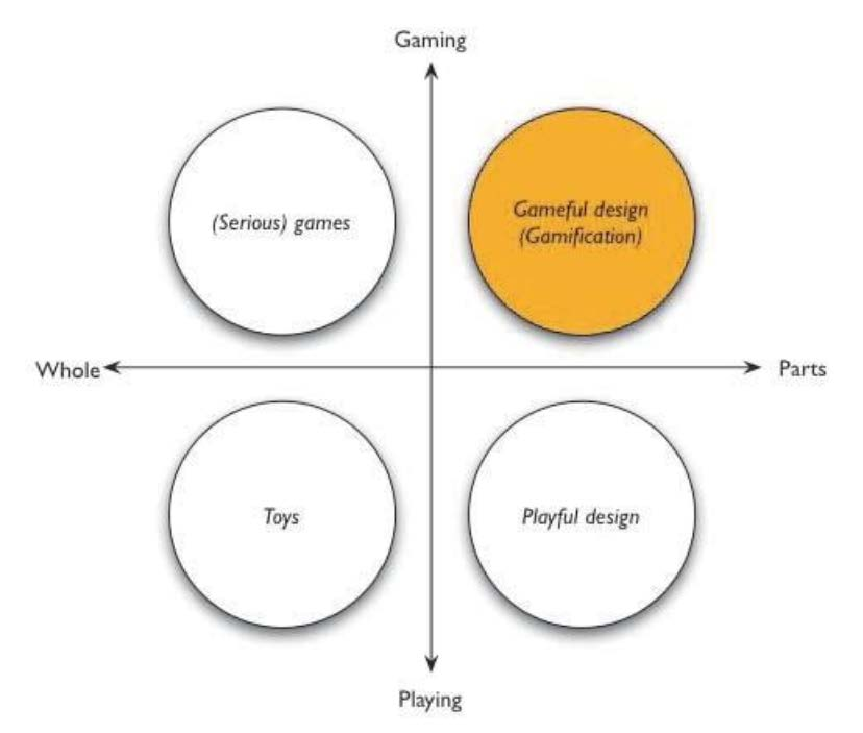
\includegraphics[scale=0.5]{Aplikovaniegamifikacie.pdf}
    \caption{Aplikovanie gamifikácie v hernom sektore\cite{deterding2011game}.}
    \label{f:gamifikacia}
\end{figure}

\subsection{Definícia cieľa hry}
Napriek veľkému počtu definícii hier sa vedci vo všeobecnosti zhodujú na tom,  že hry majú ciele\cite{zagal2019ultimate}.   Existuje množstvo dôvodov, prečo by daná hra mala motivovať hráča k ich dosiahnutiu. Napríklad motiváciou k dosiahnutiu cieľa hry je zábava, pocit úspechu a nadobudnutie vedomostí. Zatiaľ, čo pre jedného je cieľom sa pobaviť, pre toho druhého to môže byť úspešné dokončenie danej hry. Jeden z faktorov, ktorý robí hry zaujímavými je jasná definícia ich cieľa.  Na základe tohto kritéria, hry rozdeľujeme na výherné, dokončovacie alebo hry s predĺženým zážitkom.

\subsubsection{Výhra}
Jedným zo základných cieľov hry je výhra.  Ide o snahu prekonať protihráča na základe jasných ukazovateľov. Víťazstvo je považované za základný cieľ hry. Hry,  v ktorých konečným výsledkom je výhra, sú spravidla tie, v ktorých po skončení hry dochádza k vyhodnoteniu alebo posúdeniu\cite{zagal2019ultimate}. Vyhodnocovanie môže prebiehať na základe porovnávania výsledkov, na základe dosiahnutia potrebného počtu bodov,  prípadne na princípe postupného vyraďovania hráčov, až do fázy, kým sa jeden z hráčov neocitne sám. Tieto hry majú jeden spoločný cieľ, a to vyhrať.

\subsubsection{Dokončenie}
Existujú hry, ktoré majú vopred navrhnutý a určený záver (závery), ale nemajú explicitné, súťažné hodnotenie, pri ich ukončení\cite{zagal2019ultimate}. Ich cieľom je dosiahnutie konca.  Príkladom jednej z najznámejších hier takéhoto typu je GTA V (Rockstar Games 2013).  Hráči pri tomto type hier postupne prechádzajú herným systémom, až kým sa nenachádzajú vo fáze, ktorá je pre nich konečná. Do tejto kategórie patria hry bez identifikovateľného výsledku za účelom konečného cieľa dokončiť hru.

\subsubsection{Predĺženie}
Predĺženie patrí do kategórie hier, kde daná hra nemá konečný stav. Cieľom týchto hier je oddialiť ich záver nekonečným počtom životov.  Príkladom takejto hry je World of Warcraft (Blizzard 2004), ktorá je svetovým fenoménom medzi multiplayerovými hrami a držiteľom svetových ocenení.  Tieto hry nemajú koniec a o ich ukončení rozhoduje hráč. Medzi tento typ hier zaraďujeme aj hry s cieľom, ktorý však nie je možné dosiahnuť, keďže ich vývojári neustále dopĺňajú o nové úrovne. Jednou z takých hier je Don't Starve (Klei Entertainment 2013), ktorá je založená na prežití čo najväčšieho počtu dní. Hry s cieľom predĺženia nie je možné dokončiť a ich hlavným cieľom je predĺženie herného zážitku.

\subsection{Interakcia s hráčmi}

\subsection{Obmedzenie v hrách}

\subsection{Využitie zvuku v hrách}

\subsection{Logický vývoj deja}



\section{Hra}

\subsection{Vplyv hier na ľudí a ich rozvoj}

\subsection{Spoločnosti zamerané na vývoj hier}

\subsection{Rozdelenie hier podľa ich zamerania}

\subsection{Systém porovnávania určený pre hráčov}

\subsection{Vzdelávacie hry vs zábavné hry}

\section{Aplikovanie doteraz pozorovaných faktorov na hre}


%\begin{figure}[htpb]
%    \centering
%    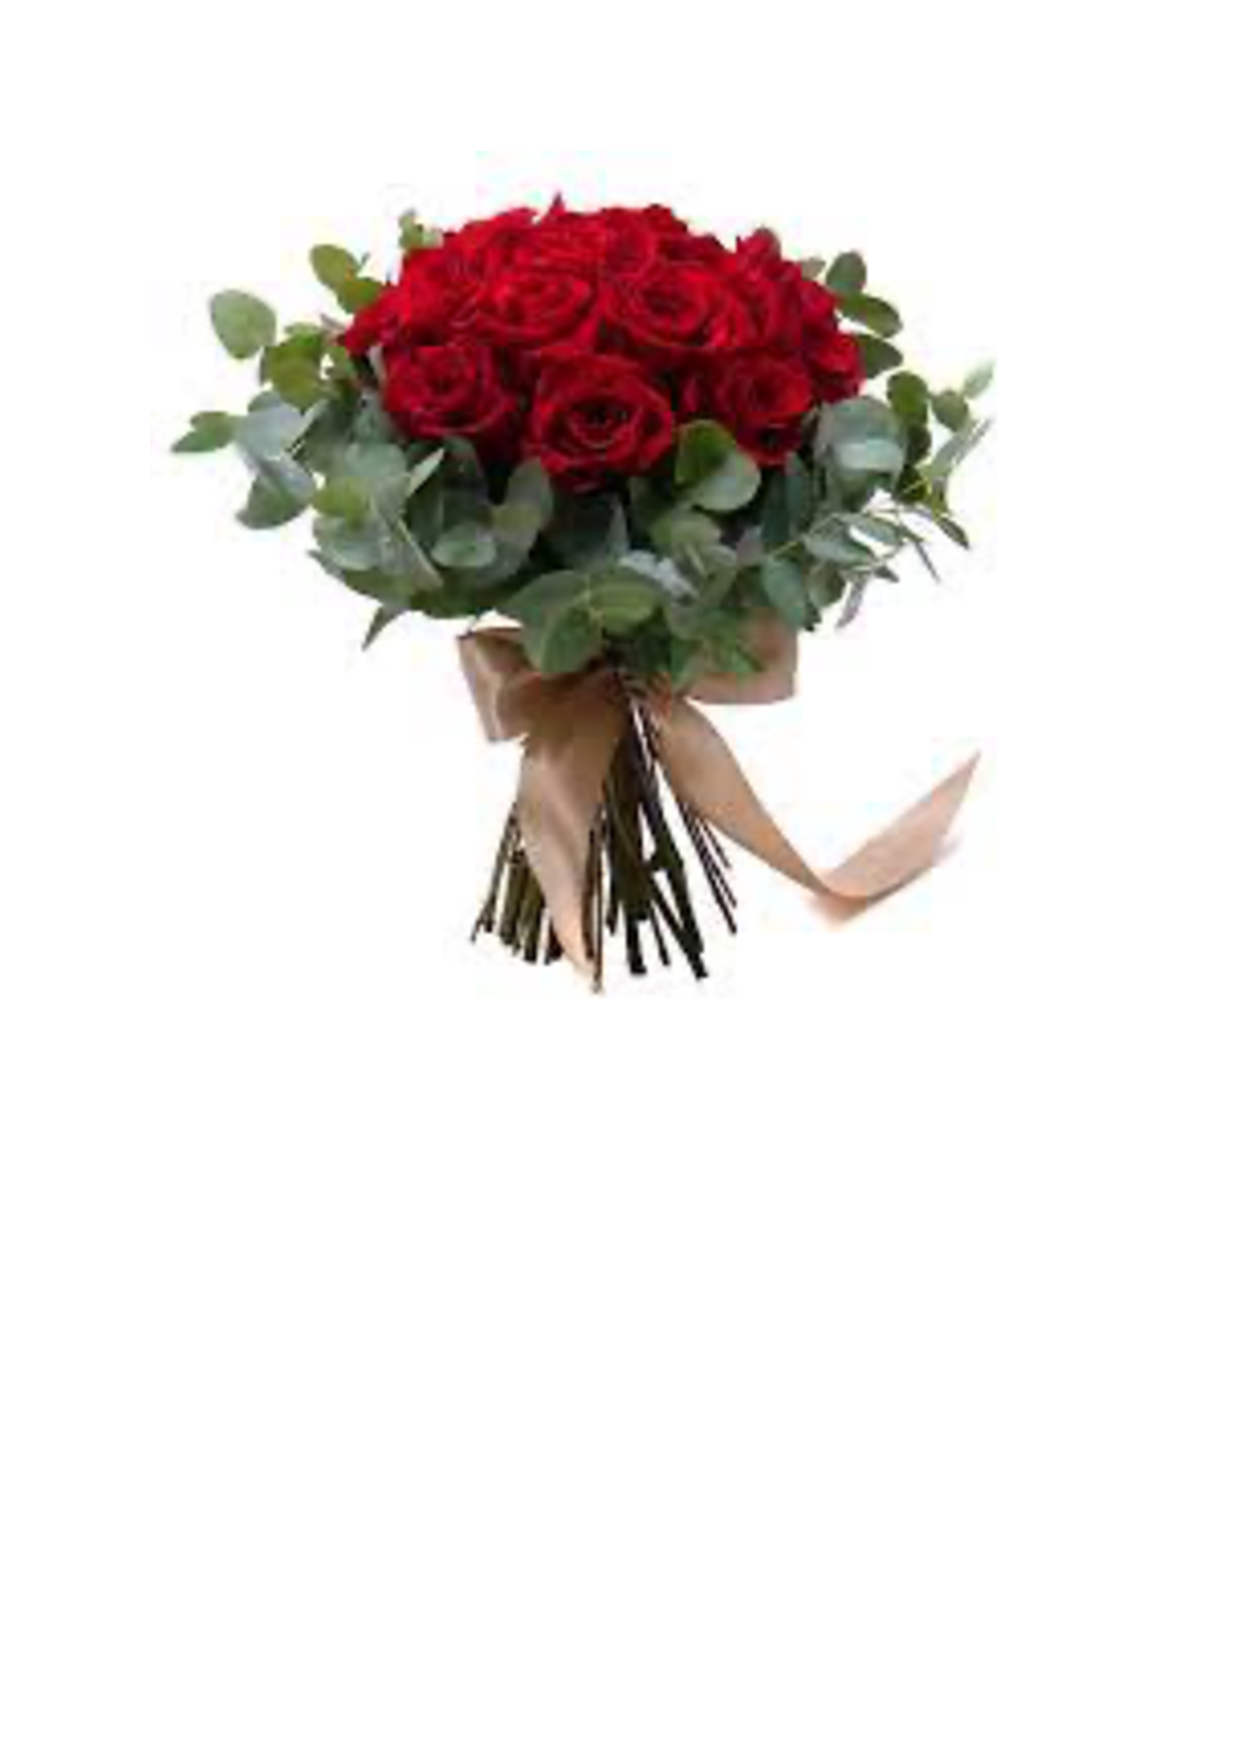
\includegraphics[scale=0.2]{Dokument1.pdf}
%    \caption{The first page of the \texttt{tikz} reference manual.}
%    \label{fig:Dokument1}
%\end{figure}


%Z obr.~\ref{f:rozhod} je všetko jasné. 



%\section{Iná časť} \label{ina}

%Základným problémom je teda\ldots{} Najprv sa pozrieme na nejaké vysvetlenie (časť~\ref{ina:nejake}), a potom na ešte nejaké (časť~\ref{ina:nejake}).\footnote{Niekedy môžete potrebovať aj poznámku pod čiarou.}

%Môže sa zdať, že problém vlastne nejestvuje\cite{Coplien:MPD}, ale bolo dokázané, že to tak nie je~\cite{Czarnecki:Staged, Czarnecki:Progress}. Napriek tomu, aj dnes na webe narazíme na všelijaké pochybné názory\cite{PLP-Framework}. Dôležité veci možno \emph{zdôrazniť kurzívou}.


%\subsection{Nejaké vysvetlenie} \label{ina:nejake}

%Niekedy treba uviesť zoznam:

%\begin{itemize}
%\item jedna vec
%\item druhá vec
%	\begin{itemize}
%	\item x
%	\item y
%	\end{itemize}
%\end{itemize}

%Ten istý zoznam, len číslovaný:

%\begin{enumerate}
%\item jedna vec
%\item druhá vec
%	\begin{enumerate}
%	\item x
%	\item y
%	\end{enumerate}
%\end{enumerate}


%\subsection{Ešte nejaké vysvetlenie} \label{ina:este}

%\paragraph{Veľmi dôležitá poznámka.}
%Niekedy je potrebné nadpisom označiť odsek. Text pokračuje hneď za nadpisom.



%\section{Dôležitá časť} \label{dolezita}




%\section{Ešte dôležitejšia časť} \label{dolezitejsia}




%\section{Záver} \label{zaver} % prípadne iný variant názvu



%\acknowledgement{Ak niekomu chcete poďakovať\ldots}


% týmto sa generuje zoznam literatúry z obsahu súboru literatura.bib podľa toho, na čo sa v článku odkazujete
\bibliography{literatura}
\bibliographystyle{plain} % prípadne alpha, abbrv alebo hociktorý iný
\end{document}
